\section[Theorie]{{Theorie\footnote[1]
{Unter Verwendung von \cite{man:v601}.}}}

\subsection{Grundlagen}
\label{sec:grundlagen}
Der Franck-Hertz-Versuch ist ein Elektronenstoßexperiment. 
In diesem Zusammenhang bedeutet das, dass Hg-Atome mit Elektronen möglichst monoenergetischer Energie beschossen werden.
Es treten sowohl elastische als auch inelastische Stöße auf.
%Die kinetische Energie $E_\text{kin}$, die die Elektronen bei den inelastischen Stößen abgeben, dient dabei als Informationsquelle.
Bei einem inelastischen Stoß wird ein Hg-Atom aus seinem Grundzustand mit der Energie $E_0$ in den ersten angeregten Zustand mit der Energie $E_1$ versetzt.
Somit entspricht die Energiedifferenz 
\begin{align}
    E_{\text{kin,vor}} - E_{\text{kin,nach}} = \frac{m_0}{2} \left(v^2_\text{vor} -v^2_\text{nach}\right) = E_1 - E_0,
    \label{eq:energiedifferenz}
\end{align}
wobei $m_0$ die Ruhemasse und $E_\text{kin}$ die kinetische Energie des Elektrons ist.
Dabei sei angemerkt, dass theoretisch auch höhere Energieniveaus möglich sind, diese allerdings mit der hier verwendeten Apparatur nicht erreicht werden.
Ferner ist es nicht möglich, die Energie der emittierten Photonen beim Wechsel zurück in den Grundzustand zu messen.
Die Energiemessung der Elektronen erfolgt mittels der Gegenfeldmethode.



\subsection{Aufbau und Ablauf des Versuchs}
\label{sec:aufbau-ablauf}
Der schematische Aufbau des Franck-Hertz-Versuchs ist in Abbildung \ref{fig:schematischer_aufbau} zu sehen.
\begin{figure}[H]
    \centering
    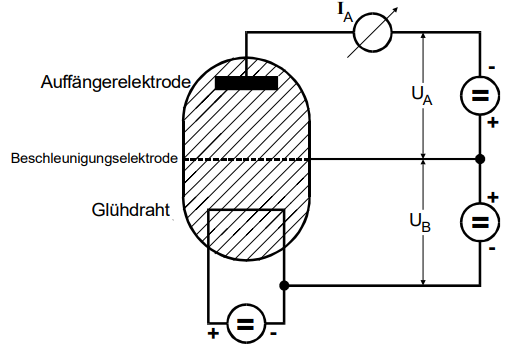
\includegraphics[height = 6.5cm]{bilder/schema.png}
    \caption{Schematischer Aufbau des Versuchs \cite{man:v601}.}
    \label{fig:schematischer_aufbau}
\end{figure}
\noindent
In dem evakuierten Glaskolben befindet sich ein kleiner Tropfen Quecksilber, welcher teilweise spontan verdampft bis sich gemäß der 
Dampfdruck-Kurve\footnote[2]{Vgl. hierzu \cite{man:v203}.} eine temperaturabhängige Sättigung $p_\text{sät}$ einstellt.
Folglich kann über die Temperatur $T$ die Dampfdichte des Quecksilbers gesteuert werden.

\noindent
In dem Gefäß befindet sich ein Glühdraht aus einem hochschmelzendem Metall, z.B. Wolfram.
Dieser wird durch eine angeschlossene Gleichspannungsquelle bis auf Rotglut erhitzt, 
sodass gemäß des glühelektrischen Effektes\footnote[3]{Vgl. hierzu \cite{man:v504}.} Elektronen aus dem Draht gelöst werden.
Bei gegebener Temperatur wird dieser Effekt dadurch verstärkt, dass der Draht mit dem Oxid eines Erdalkalimetalls bestrichen wird,
welches eine niedrigere Austrittsarbeit\footnotemark[3] als Wolfram hat.

\noindent
Außerdem befindet sich eine netzförmige Beschleunigungselektrode im Gefäß, die von außen mit einer positiven Gleichspannung $U_\text{B}$
betrieben wird.
Durch das entstehende elektrische Feld werden die Elektronen zur Elektrode hin beschleunigt.
Falls die Elektronen vorher in Ruhe waren, gilt für sie nach der Beschleunigungsstrecke
\begin{align}
    \frac{1}{2} m_0 v^2_\text{vor} = e_0 U_\text{B}, 
    \label{eq:beschleunigung}
\end{align}
\noindent wobei $e_0$ die Elementarladung ist.

\noindent
Zum Messen des Auffängerstroms $I_\text{A}$ befindet sich eine Auffängerelektrode hinter der Beschleunigungselektrode,
die an eine Gegenspannungsquelle $U_\text{A}$ angeschlossen ist und ein Gegenfeld erzeugt.
Somit können nur solche Elektronen mit Geschwindigkeit $v_\text{z}$ in $z$-Richtung die Auffängerelektrode erreichen, die 
\begin{align}
    \frac{1}{2} m_0 v^2_\text{z} \geq e_0 U_\text{A}
    \label{eq:v-kriterium}
\end{align}
erfüllen.

\noindent
Wie in Abschnitt \ref{sec:grundlagen} beschrieben finden sowohl elastische als auch inelastische Stöße zwischen Elektronen und Hg-Atomen statt.
Dabei gibt es je nach Elektronenenergie zwei Fälle.
Falls die kinetische Energie der Elektronen nicht ausreicht, kommt es ausschließlich zu elastischen Stößen.
Aufgrund des großen Massenunterschieds zwischen Elektron und Hg-Atom ist die abgegebene Energie des Elektrons vernachlässigbar gering,
obwohl es enorme Richtungsänderungen erfahren kann.
Falls $U_\text{B}$ so weit erhöht wird, 
dass die kinetische Energie der Elektronen mindestens der Energiedifferenz $E_1 - E_0$ aus Formel \eqref{eq:energiedifferenz} entspricht,
kann das Hg-Atom durch das Elektron in seinen ersten angeregeten Zustand versetzt werden.
Nach einer Relaxationszeit der Größenordnung $\qty{10}{\nano\second}$ springt das Atom in seinen Grundzustand zurück.
Dabei wird ein Photon mit Frequenz $\nu$ der und der Energie 
\begin{align}
    E_1 - E_0 = h \nu
    \label{eq:photon}
\end{align}
emittiert, wobei $h$ das Plancksche Wirkungsquantum ist.

\noindent
Wird $I_\text{A}$ in Abhängigkeit von $U_\text{B}$ bei konstantem $U_\text{A}$ gemessen, 
so ergibt sich im Idealfall ein Plot wie in Abbildung \ref{fig:f-h-ideal}.
Bei steigendem $U_\text{B}$ wird $U_\text{A}$ an einer gewissen Stelle überschritten, sodass $I_\text{A}$ stark ansteigt.
Sobald die Energiedifferenz $E_1 - E_0$ erreicht wird, treten inelastische Stöße auf und die Elektronen geben eben diesen Energiebetrag ab.
Das führt dazu, dass gar keine Elektronen die Auffängerelektrode erreichen, weshalb $I_\text{A} = 0$ gilt.
Von da aus wiederholt sich der Prozess periodisch, wenn $U_\text{B}$ erhöht wird, da die Elektronen nach dem Stoß auf der Beschleunigungsstrecke weitere Energie aufnehmen. 
Anhand der vorhanden Peaks im Plot kann also die Anregungsenergie $E_1 - E_0$ bzw. ein ganzzahliges Vielfaches der Energie abgelesen werden.
Es gibt also die Relation 
\begin{align}
    U_1 = \frac{1}{e_0} \left(E_1 - E_0\right)
\end{align}
für den Abstand $U_1$ der Maxima und der Energiedifferenz.

\begin{figure}[H]
    \centering
    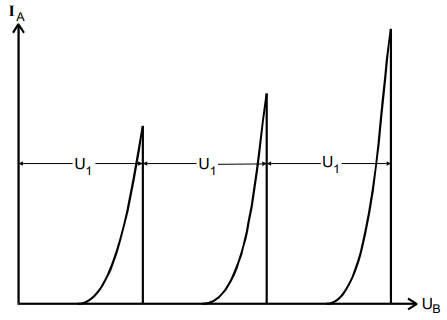
\includegraphics[height = 6.5cm]{bilder/franck-hertz-ideal.png}
    \caption{Die ideale Franck-Hertz-Kurve \cite{man:v601}.}
    \label{fig:f-h-ideal}
\end{figure}
\noindent

\subsection{Störeinflüsse auf die ideale Franck-Hertz-Kurve}
Die ideale Franck-Hertz-Kurve \ref{fig:f-h-ideal} kann im Realfall nicht erreicht werden, was mit folgenden Nebeneffekten zusammenhängt.

\subsubsection{Kontaktpotential $K$}
Haben der Glüdraht und die Beschleunigungselektrode ungleiche Austrittsarbeiten, kommt es zu einem effektiven Beschleunigungspotential $U_\text{B,eff}$,
welches von der angelegten Spannung $U_\text{B}$ verschieden ist.
Die Austrittsarbeit des Materials des Glühdrahtes $\phi_\text{G}$ ist deutlich kleiner als die der Beschleunigungselektrode $\phi_\text{B}$,
damit auch bei kleinen Temperaturen $T$ hohe Emissionsraten vorliegen.
Das Potentialgefälle ist in Abbildung \ref{fig:potential} zu sehen.
Zur Beschreibung eben dieses Gefälles wird das Kontaktpotential 
\begin{align}
    K = \frac{1}{e_0} \left(\phi_\text{B}- \phi_\text{G}\right)
    \label{eq:kontaktpotential}
\end{align}
eingeführt, sodass sich nach Abbildung \ref{fig:potential} 
\begin{align}
    U_\text{B,eff} = U_\text{B} - K
    \label{eq:u-b-eff}
\end{align}
ergibt.

\begin{figure}[H]
    \centering
    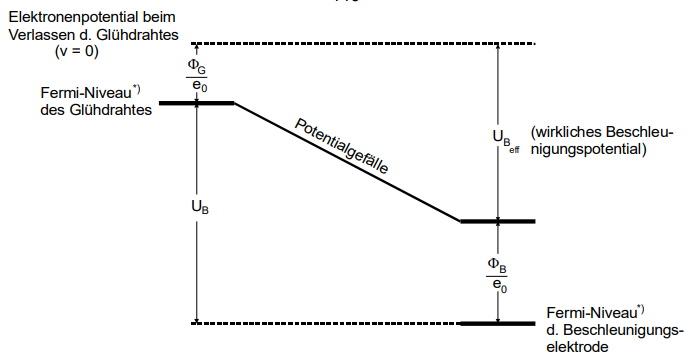
\includegraphics[height = 6.5cm]{bilder/potential.png}
    \caption{Eine Darstellung des Potentialgefälles der Elektroden \cite{man:v601}.}
    \label{fig:potential}
\end{figure}
\noindent

\subsubsection{Das Energiespektrum der Elektronen}
Die Elektronen im Inneren eines Metalles unterliegen der Fermi-Dirac-Verteilung, d.h. sie haben unterschiedliche Energien \cite{man:v504}.
Somit treten sie beim glühelektrischen Effekt mit unterschiedlichen Anfangsgeschwindigkeiten aus dem Draht.
Nach dem Durchlaufen der Beschleunigungsstrecke liegt demnach eine kontinuierliche Energieverteilung vor.
Die inelastischen Stöße finden also nicht bei einem festen $U_\text{B}$ sondern bei einem endlichen Bereich um diese statt.
Dadurch wird der Anstieg der Kurve zum Maximum hin verringert.
Im Anschluss wird die Kurve stetig auf ein lokales Minimum sinken.

\noindent
Die elastischen Stöße zwischen Glühdraht und Beschleunigungselektrode tragen aufgrund der geringen Energieabgabe nicht signifikant zu einer Veränderung der Kurve bei.
Finden diese Stöße jedoch zwischen Beschleunigungs- und Auffängerelektrode statt, entsteht eine Verteilung von $v_\text{z}$ (vgl. Abschnitt \ref{sec:aufbau-ablauf}).
Dadurch wird die Kurve abgeflacht und gestreckt.

\subsubsection{Der Dampfdruck}
\label{sec:dampfdruck}
Damit ausreichend viele Stöße auftreten können, muss die mittlere freie Weglänge $\bar{w}$ klein im Vergleich zum Abstand $a$ zwischen Kathode und Beschleunigungselektrode sein.
Es sollte etwa ein Faktor 1000 bis 4000 vorliegen.
Hier beträgt $a = \qty{1}{\cm}$.
Dabei gilt der Zusammenhang 
\begin{align}
    \bar{w} = \frac{0.0029}{p_\text{sät}}
\end{align} 
zwischen $\bar{w}$ in Zentimetern und dem Sättigungsdampfdruck $p_\text{sät}$ in Millibar.
Die Dampfdruck-Kurve von Hg kann gemäß 
\begin{align}
    p_\text{sät}(T) = \num{5.5} \cdot 10^7 \cdot \exp\left(-\frac{6876}{T}\right)
\end{align}
in Abhängigkeit der Temperatur $T$ bestimmt werden, wobei $p_\text{sät}$ hier in Millibar und $T$ in Kelvin angegeben wird.
Der zugehörige Plot ist in Abbildung \ref{fig:dampfdruck} zu sehen.
% Somit kann die Temperatur $T$ bestimmt werden, bei der der Franck-Hertz-Effekt eintritt.

\begin{figure}[H]
    \centering
    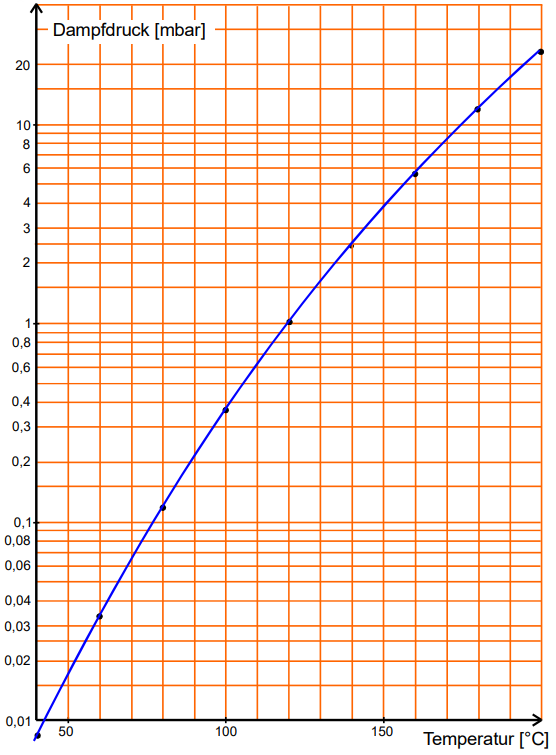
\includegraphics[height = 10cm]{bilder/dampfdruck.png}
    \caption{Die Dampfdruck-Kurve von Hg \cite{man:v601}.}
    \label{fig:dampfdruck}
\end{figure}

\noindent
Es gibt also ein Dampfdruckintervall, in dem die Apparatur am besten arbeitet.
Liegt $p_\text{sät}$ unterhalb, ist es zunehmend unwahrscheinlich, dass Stöße stattfinden.
Ist in diesem Fall $U_\text{B}$ groß genug, würde die kinetische Energie der Elektronen theoretisch auch für höhere Anregungszustände ausreichen.
Tatsächlich ist die Wechselwirkungswahrschienlichkeit hier zu klein.
Wird $p_\text{sät}$ zu groß gewählt, treten mehr elastische Stöße auf.
Durch die starken Richtungsänderungen nimmt die Zahl der Elektronen, die die Auffängerelektrode erreichen deutlich ab.


\subsection{Aufbau der Elektronenhülle}
Der Übergang vom Grund- in den ersten angeregten Zustand bei Atomen mit einer hohen Protonenanzahl z wie Hg ist relativ unwahrscheinlich,
da hierfür ein Umklappen des Elektronenspins erforderlich ist.
Bei einer kleinen Anzahl z ist der Übergang fast unmöglich.
Wenn allerdings ein Elektron das Atom anregt, so wie es bei diesem Versuch der Fall ist,
wird die Wahrscheinlichkeit stark erhöht.
Das hängt damit zusammen, dass das Elektron, welches mit dem Atom stößt, eines von zweien Schalenelektronen mit entgegengesetzter Spinrichtung ersetzt.